\chapter{Музыкальные композиции}
\label{ch:musical-composition}
Глава посвящена исследованию музыкальных композиций. 
С помощью SPARQL-запросов, вычисляемых на объектах типа <<музыкальная композиция>> в~Викиданных, 
получены списки музыкальных композиций, список наиболее плодовитых композиторов, 
найдены популярные музыкальные жанры. 
Получен список музыкальных произведений в Викиданных, 
для~которых будет законной загрузка их аудиозаписей на~Викисклад, поскольку истек срок копирайта.

\section{Число <<музыкальных композиций>> и жанры}

В запросах будем работать с~объектами \wdqName{<<музыкальное произведение/композиция>>}{105543609}. 
Получим список всех таких объектов с помощью запроса~\ref{lst:musical_composition}.

\begin{lstlisting}[ 
    language=SPARQL,
    caption={\href{https://w.wiki/9vq3}{Список всех  музыкальных композиций}\protect\footnotemark},
    label=lst:musical_composition,
    texcl,
    numbers=none
    ]
# List of all musical compositions
SELECT (COUNT(?music) AS ?count) WHERE
{
  ?music wdt:P31 wd:Q105543609. # is musical composition
}
\end{lstlisting}%
\footnotetext{Получено: \num{5495} записей на 2017 год, 107~тыс.~--- на~2022 год и 160 тыс.~--- на~2024 год. 
        Ссылка на~SPARQL-запрос: \href{https://w.wiki/9vq3}{https://w.wiki/9vq3}.}

Наиболее полными и проработанными примерами музыкальных композиций на Викиданных являются: 
\wdqName{<<Волшебная флейта>>}{5064}, 
\wdqName{<<К Элизе>>}{11980}, 
\wdqName{<<Реквием>>}{207875}, 
\wdqName{<<Маленькая ночная серенада>>}{12025}, 
\wdqName{<<Соната си синор>>}{63681379}.

В~2017 году по запросу~\ref{lst:musical_composition} найдено \num{5,5} тыс. музыкальных композиций, 
в 2022 году~--- 107 тыс., в~2024~--- 160 тыс. 
Увеличение числа композиций в 2022 году, по сравнению с 2017 годом, связано с~тем, 
что в~2017 году в~запросе~\ref{lst:musical_composition} мы искали экземплярами 
объекта \wdqName{composed musical work}{207628}, а с 2022 мы 
переключились на поиск объектов \wdqName{musical work/composition}{105543609} 
(<<музыкальное произведение/композиция>>). 

%При поиске подклассов объекта <<музыкальное произведение/композиция>> можно найти такие жанры, как: 
%\wdqName{<<песня>>}{7366}, 
%\wdqName{<<духовная песня>>}{856713}, 
%\wdqName{<<гимн>>}{484692}. 
%Более подробно анализ музыкальных жанров представлен в~разделе 
%<<Количество музыкальных произведений по~жанрам>> на~с.~\pageref{chapter:Number-of-musical-works-by-genre}.


\begin{marginfigure}[0\baselineskip]
	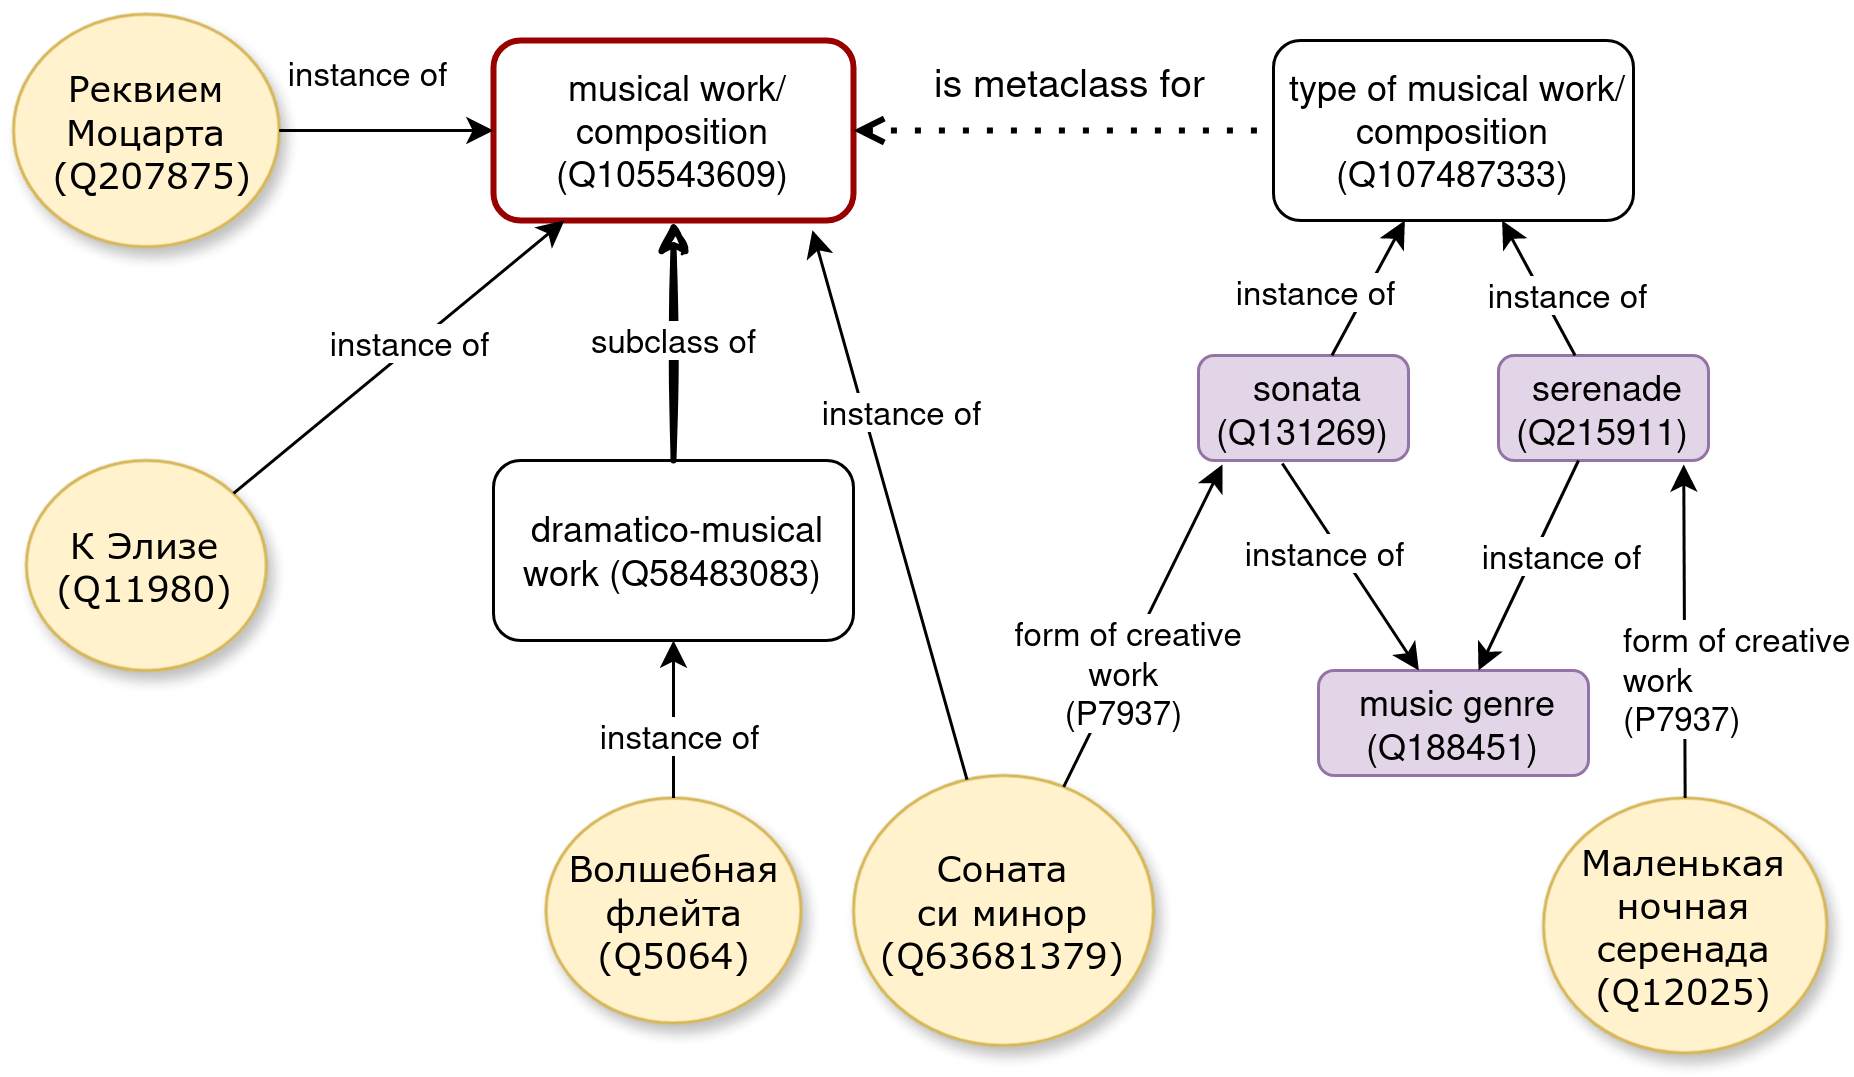
\includegraphics[width=1\textwidth]{./chapter/musical_composition/hierarchy_of_music_classes_WD_2023.png}
	\caption[Иерархия музыкальных классов]{Фрагмент иерархии музыкальных классов в Викиданных, 2023 год}%
	\label{fig:hier-music}%
\end{marginfigure}
%
Музыкальные объекты Викиданных связаны между собой множеством отношений 
и~образуют сложную иерархию (рис.~\ref{fig:hier-music}). 
Вот некоторые из этих отношений: 
\begin{enumerate}
        \item <<\wdProperty{31}{экземпляр}>>~--- instance of;
        \item <<\wdProperty{279}{подкласс от}>>~--- subclass of;
        \item <<\wdProperty{8225}{метакласс для}>>~--- is metaclass for;
        \item <<\wdProperty{7937}{форма творческой работы}>>~--- form of creative work.
\end{enumerate}

Категории в вики-проектах представляют собой \emph{несколько пересекающихся иерархий} 
(несколько <<деревьев>> в терминах теории графов). 
Несмотря на то, что категории содержат только один вид отношений 
(родитель-ребёнок или общее-частное), 
отношения между объектами Викиданных во многом близки таковым между категориями. 
Например, на~рис.~\ref{fig:hier-music} видно 
\emph{несколько пересекающихся деревьев} с~корнями в~следующих вершинах:  
        \wdqName{musical work/composition}{105543609}, 
        \wdqName{music genre}{188451}, 
        \wdqName{type of musical work/composition}{107487333}.


С помощью запроса~\ref{lst:music_in_each_subclass} найдём количество объектов 
в~каждом подклассе объекта \wdqName{<<музыкальная композиция>>}{105543609}. 

\marginnote[3\baselineskip]{%
        \label{question:music_comp}
        \MarginQuestion
        В 9 подклассов \wdqName{<<музыкальных композиций>>}{105543609}, 
        полученных по~запросу~\ref{lst:music_in_each_subclass}, 
        входят объекты \wdqName{incipit}{1161138} (<<начальные слова>>) 
                     и~\wdqName{Masque}{1907293} (<<маска>>), то есть это не~музыкальные вещи. 
        Как исключить эти <<слова>> и <<маску>> и оставить только музыкальные объекты?

        См. ответ %~\ref{lst:music_in_each_subclas_2} 
        на~с.~\pageref{answer:music_in_each_subclas_filter}.
}

\begin{lstlisting}[ 
    language=SPARQL,
    caption={\href{https://w.wiki/9U7w}
                  {Количество объектов в подклассах музыкальных композиций}\protect\footnotemark},
    label=lst:music_in_each_subclass,
    xleftmargin=18pt,
    numbers=left,
    ]
# Number of musical works in each subclass
SELECT ?type (COUNT(?music) AS ?count) ?typeLabel WHERE 
{                      # subclass of musical composition
                 ?type wdt:P279* wd:Q105543609.      
  ?music wdt:P31 ?type.
         # instance of this subclass
  SERVICE wikibase:label { bd:serviceParam wikibase:language "ru, en" }
}
GROUP BY ?type ?typeLabel
ORDER BY DESC (?count)
\end{lstlisting}%
\footnotetext{Получено: 9 подклассов музыкальных композиций на 2024 год. Ссылка на SPARQL-запрос: \href{https://w.wiki/9U7w}{https://w.wiki/9U7w}.}


В этом запросе~\ref{lst:music_in_each_subclass} 
мы используем только левую часть рис.~\ref{fig:hier-music}, 
а~именно объект \wdqName{musical work/compo\-sition}{105543609}. 
Поэтому в подклассах нет ни сонаты, ни серенады.

Теперь напишем два запроса таким образом, 
чтобы по~запросу~\ref{lst:Number_of_types_of_musical_works_1} получить 
список \wdqName{<<типов музыкальных произведений>>}{107487333}, 
а~по~запросу~\ref{lst:Number_of_types_of_musical_works_2}~--- 
список \wdqName{<<музыкальных жанров>>}{188451}. 
Эти запросы задействуют правую часть рис.~\ref{fig:hier-music}. 
В~соответствии с~этим рисунком в~результатах обоих запросов будут присутствовать такие 
музыкальные жанры, как соната и~серенада.

\begin{lstlisting}[ 
    language=SPARQL,
    caption={\href{https://w.wiki/9U8o}
                  {Список \wdqName{<<типов музыкальных произведений>>}{107487333}}\protect\footnotemark},
    label=lst:Number_of_types_of_musical_works_1,
    texcl,
    ]
# Number of types of musical works
SELECT ?type ?typeLabel WHERE 
{                # type of musical work
  ?type wdt:P31 wd:Q107487333.      
  SERVICE wikibase:label { bd:serviceParam wikibase:language "ru, en" }
}
\end{lstlisting}%
\footnotetext{Получено: 280 типов музыкальных работ на 2024 год. Ссылка на SPARQL-запрос: \href{https://w.wiki/9U8o}{https://w.wiki/9U8o}.}

\begin{lstlisting}[ 
    language=SPARQL,
    caption={\href{https://w.wiki/9vuZ}
                  {Список \wdqName{<<музыкальных жанров>>}{188451}}\protect\footnotemark},
    label=lst:Number_of_types_of_musical_works_2,
    texcl,
    ]
# Number of music genres
SELECT ?type ?typeLabel WHERE 
{                #  music genre
  {?type wdt:P31 wd:Q188451} .
  SERVICE wikibase:label { bd:serviceParam wikibase:language "ru, en" }
}
\end{lstlisting}%
\footnotetext{Получено: 5809 музыкальных жанров на 2024 год. Ссылка на SPARQL-запрос: \href{https://w.wiki/9vuZ}{https://w.wiki/9vuZ}.}

Объединим типы музыкальных работ и музыкальные жанры 
в~запросе~\ref{lst:Number_of_genres_and_types_of_musical_works}. 
Для объединения утверждений в~строках 4~и~5~служит команда \lstinline|UNION|. 
Чтобы объекты не~повторялись, 
укажем в~команде \lstinline|SELECT| параметр \lstinline|DISTINCT| (строка~2). 
Дубликатов оказалось полтора процента. 

\newpage
        \lstset{escapeinside={(*@}{@*)}}
        \sethlcolor{pink}
        \index{SPARQL!DISTINCT}
        \index{SPARQL!UNION}
\begin{lstlisting}[ 
    language=SPARQL,
    caption={\href{https://w.wiki/9nSA}
                  {Суммарное число музыкальных композиций в подклассах}\protect\footnotemark},
    label=lst:Number_of_genres_and_types_of_musical_works,
    xleftmargin=18pt,
    numbers=left,
    ]
# List of genres and types of musical works
SELECT (*@\hl{DISTINCT}@*) ?type ?typeLabel WHERE 
{                # type of musical work/composition
  {?type wdt:P31 wd:Q107487333} (*@\hl{UNION}@*)
  {?type wdt:P31 wd:Q188451} .
                 # music genre
  SERVICE wikibase:label { bd:serviceParam wikibase:language "ru, en" }
}
\end{lstlisting}%
\footnotetext{Получено: 6017 музыкальных типов и жанров на 2024 год. Ссылка на~SPARQL-запрос: \href{https://w.wiki/9nSA}{https://w.wiki/9nSA}.}

Допишем запрос~\ref{lst:Number_of_genres_and_types_of_musical_works}, 
чтобы он подсчитал число музыкальных произведений (без дубликатов), 
которые имеют такой музыкальный тип или жанр. 
Для этого возьмём экземляры выбранного типа или жанра в~строке~6 
запроса~\ref{lst:NPiecesOfMusicForEachGenre}.
\begin{lstlisting}[ 
    language=SPARQL,
    caption={\href{https://w.wiki/9pfM}
                  {Число музыкальных композиций в каждом из жанров и типов}\protect\footnotemark},
    label=lst:NPiecesOfMusicForEachGenre,
    xleftmargin=18pt,
    numbers=left,
    ]
# List of number of pieces of music, grouped by genre and type
SELECT (COUNT(DISTINCT ?music) AS ?num) ?type ?typeLabel WHERE
{                
  {?type wdt:P31 wd:Q107487333} UNION # type of musical work/composition
  {?type wdt:P31 wd:Q188451}.         # music genre
  (*@\hl{?music wdt:P31 ?type.}@*) # music of this type or genre
  SERVICE wikibase:label { bd:serviceParam wikibase:language "ru, en" }
}
GROUP BY ?type ?typeLabel
\end{lstlisting}%
\footnotetext{Получено: 254 жанра и типа музыкальных произведений на 2024 год. Ссылка на~SPARQL-запрос: \href{https://w.wiki/9pfM}{https://w.wiki/9pfM}.}

Суммируем число музыкальных композиций, входящих в различные жанры и музыкальные типы, 
с~помощью двух вложенных команд \lstinline|SELECT| в~запросе~\ref{lst:TotalPiecesMusicAllGenres}. 
% 
Внутренний \lstinline|SELECT| (строки 3--8)~--- это тот~же запрос~\ref{lst:NPiecesOfMusicForEachGenre}, 
который мы разобрали выше, но без ненужных здесь меток \lstinline|?typeLabel|. 
Во~внутреннем блоке \lstinline|SELECT| мы обходим все музыкальные типы и жанры, 
записывая в~переменную \lstinline|?num| число <<музык>> в выбранном жанре. 
% 
Функция \lstinline|SUM()| во~внешней команде \lstinline|SELECT| 
суммирует эти числа \lstinline|?num| в~переменную \lstinline|?total|. 
С~помощью запроса~\ref{lst:TotalPiecesMusicAllGenres} получили около 30~тыс. музыкальных композиций.


\newpage
\begin{lstlisting}[ 
    language=SPARQL,
    caption={\href{https://w.wiki/9ps2}
                  {Суммарное число музыкальных композиций по всем жанрам и типам}\protect\footnotemark},
    label=lst:TotalPiecesMusicAllGenres,
    xleftmargin=18pt,
    numbers=left,
    ]
# Total number of pieces of music of various genres and types
SELECT ((*@\hl{SUM}@*)(?num) AS (*@\hl{?total}@*)) WHERE {
  SELECT (COUNT(DISTINCT ?music) AS (*@\hl{?num}@*))) WHERE
  {                
    {?type wdt:P31 wd:Q107487333} UNION # type of musical work/composition
    {?type wdt:P31 wd:Q188451}.         # music genre
    ?music wdt:P31 ?type. # music of this type or genre
  }
  GROUP BY ?type
}
\end{lstlisting}%
\footnotetext{Получено: \lstinline|total|=\num{27530} на 2024 год. 
              Ссылка на~SPARQL-запрос: \href{https://w.wiki/9ps2}{https://w.wiki/9ps2}.}


Теперь подсчитаем общее суммарное число музыкальных произведений с учётом музыкальных композиций в подклассах. 
Для этого добавим в~запрос~\ref{lst:music_in_each_subclass} команду \lstinline|SUM()| в~строку~2 
и~удалим лишние строки, чтобы получить запрос~\ref{lst:TotalMusicAllSubclasses}.


\begin{lstlisting}[ 
    language=SPARQL,
    caption={\href{https://w.wiki/9tua}
                  {Суммарное число музыкальных произведений 
                   с~учётом музыкальных композиций в~подклассах}\protect\footnotemark},
    label=lst:TotalMusicAllSubclasses,
    xleftmargin=18pt,
    numbers=left,
    ]
# The total number of musical works for all subclasses 
SELECT (SUM(?count) AS ?sum) WHERE{
  SELECT (COUNT(?music) AS ?count) WHERE {               
    ?type wdt:P279* wd:Q105543609. # subclass of musical work/composition
       ?music wdt:P31 ?type		        # instance of this subclass
	FILTER (?type != wd:Q1161138 && ?type != wd:Q1907293)
  }       
}
\end{lstlisting}%
\footnotetext{Получено: 145~тыс. музыкальных произведений на 2022 год, 
    164~тыс. на 2023 год и 170~тыс. на 2024 год. 
    Ссылка на~SPARQL-запрос: \href{https://w.wiki/9tua}
                                  {https://w.wiki/9tua}.}

Как и в задаче на с.~\pageref{question:music_comp}, нам необходимо исключить появление 
объектов ``incipit (wd:Q1161138)'' и ``Masque (wd:Q1907293)'' в результатах запроса. 
Для этого воспользуемся ответом на с.~\pageref{answer:music_in_each_subclas_filter}. 
С помощью строки 6 в запросе~\ref{lst:TotalMusicAllSubclasses} мы избавимся от нежелательных результатов. 
Всего таких оказалось 10. 

Можно записать этот код ещё короче. 
Переменная \lstinline|?type| нам не нужна, 
поэтому заменим её на \emph{безымянную переменную}, \index{SPARQL![]!безымянная переменная}
а~строки 5 и 6 поменяем местами, 
получаем запрос~\ref{lst:TotalMusicAllSubclasses_up}.


\newpage
\begin{lstlisting}[ 
    language=SPARQL,
    caption={\href{https://w.wiki/9Td7}
                  {Суммарное число музыкальных произведений с~учётом музыкальных композиций 
                  в~подклассах (безымянная переменная)}\protect\footnotemark},
    label=lst:TotalMusicAllSubclasses_up,
    texcl,
    numbers=none
    ]
# Total number of musical works for all subclasses
SELECT (SUM(?count) AS ?sum) WHERE{
  SELECT (COUNT(?music) AS ?count) WHERE {
    ?music wdt:P31   # instance of
          [wdt:P279* wd:Q105543609].  # subclass of musical work/composition
  }       
}
\end{lstlisting}%
\footnotetext{Этот запрос идентичен предыдущему по результатам, то~же число результатов. 
Ссылка на~SPARQL-запрос: \href{https://w.wiki/9Td7}{https://w.wiki/9Td7}.}

Таким образом, имеем два способа перечисления музыкальных объектов: 
\begin{enumerate}
    \item через экземпляры музыкальных жанров и типов в~запросе~\ref{lst:TotalPiecesMusicAllGenres}, 
        получено около 30~тыс. объектов на 2024 год. 

    \item через экземпляры подклассов музыкальных композиций в~запросе~\ref{lst:TotalMusicAllSubclasses_up}, 
        получено 170~тыс. объектов на 2024 год.
\end{enumerate}

Предложим задачи для самостоятельной работы. 
Насколько велико пересечение этих двух множеств в~30 и~170~тыс.? 
Если пересечение относительно мало, то напишите запрос, 
который будет объединять эти два множества без повторений. 





\section{Сколько старой и новой музыки (до и начиная с 2018 года) есть в Викиданных}

По сравнению с~2022 годом, когда было получено 107~тыс. записей в~запросе~\ref{lst:musical_composition}, 
число записей в~2024 году увеличилось в~половину. 
Это связано с~тем, что за~два года были созданы и добавлены в~Викиданные новые музыкальные произведения, 
а~также были добавлены старые, не~учтённые ранее. 
Напишем скрипт~\ref{lst:music2018-2024} и~посмотрим сколько 
старых, то есть созданных до 2018 года, и новых, созданных в 2018--2024 годах, 
музыкальных произведений присутствует в~Викиданных.

В первой версии запроса~\ref{lst:music2018-2024} 
(см. запрос \href{https://w.wiki/9pxA}{https://w.wiki/9pxA}) 
мы использовали вместо строк 6--7 тяжёлую конструкцию, но в одну строчку: 
\lstinline|FILTER(?date > "2018-01-01T00:00:00Z"^^xsd:dateTime)|. 
%
В варианте кода, представленном в листинге запроса~\ref{lst:music2018-2024}, 
мы получаем более читаемый код с~использованием команды \lstinline|BIND| в строке 6 
и~переменной \lstinline|?year| в строках 6--7.


\newpage
\begin{lstlisting}[ 
    language=SPARQL,
    caption={\href{https://w.wiki/9wHp}
                  {Количество музыкальных композиций, созданных в 2018--2024 годы}\protect\footnotemark},
    label=lst:music2018-2024,
    xleftmargin=18pt,
    numbers=left,
    ]
# Number of musical compositions created in 2018-2024
SELECT (SUM(?count) AS ?sum) WHERE{
  SELECT (COUNT(?music) AS ?count) WHERE{
    ?music wdt:P31 wd:Q105543609;  # is musical work/composition
           wdt:P577 ?date.         # has a publication date
    (*@\hl{BIND}@*)(YEAR(?date) AS (*@\hl{?year}@*))
    FILTER((*@\hl{?year}@*)) > 2017)
  }
}
\end{lstlisting}%
\footnotetext{Получено: \num{5403} музыкальных произведений за 2018--2024 годы. Ссылка на SPARQ-запрос: \href{https://w.wiki/9wHp}{https://w.wiki/9wHp}.}


Запрос~\ref{lst:TotalMusicAllSubclasses_up} 
возвращает 170 тыс. музыкальных произведений, которые могут иметь или не~иметь дату публикации. 
В~запросе~\ref{lst:music2018-2024} в~строке~5 
мы требуем обязательного наличия свойства \wdProperty{577}{<<дата публикации>>} у~музыкального произведения.
Таких произведений с~заполненной датой публикации и 
с~отсутствием ограничений на год публикации 
(строка~7 в~запросе~\ref{lst:music2018-2024} закомментированна) 
найдено 55 тыс., 
то есть примерно в~3~раза меньше. 
Если включена фильтрация на~год публикации (строка~7), 
то получаем 5.4 тыс. новых произведений, созданных в~2018--2024 годах, имеющих объекты в Викиданных. 
Получается, что <<новых>> музыкальных произведений, созданных после 2017 года,  
около 3\,\% (5.4 тыс.) от всех музыкальных произведений в Викиданных (170 тыс.).






\section{Количество музыкальных произведений по годам}

Подсчитаем количество музыкальных произведений 
со второй половины XIX века до настоящего времени 
с~помощью запроса~\ref{lst:MusicEvery10Years}. 
Этот запрос строит рис.~\ref{fig:diagram_10_years}, где 
указано число созданных произведений по десятилетиям. 


\index{SPARQL!wikibase!isSomeValue}
\begin{lstlisting}[ 
    language=SPARQL,
    caption={\href{https://w.wiki/9wJC}
                  {Количество музыкальных произведений, создаваемых каждое десятилетие}\protect\footnotemark},
    label=lst:MusicEvery10Years,
    xleftmargin=18pt,
    numbers=left,
    ]
# The number of musical compositions for every 10 years
#defaultView:BarChart
SELECT (STR(?date) AS ?date_str) (COUNT(?composition) AS ?count) WHERE {
  ?composition wdt:P31 wd:Q105543609; # is musical work/composition
               wdt:P86 ?composer;     # has a composer
               wdt:P577 ?publication. # has a publication date
  BIND(YEAR(?publication) AS ?date)
  BIND((FLOOR(?date / 10 )) * 10  AS ?year)
  FILTER(1850 < ?year && ?year < 2030)
  FILTER (!wikibase:isSomeValue(?publication)) # field "date" must be filled
}
GROUP BY ?date
ORDER BY (?date)
\end{lstlisting}%
\footnotetext{Ссылка на SPARQL-запрос: \href{https://w.wiki/9wJC}{https://w.wiki/9wJC}.}


\begin{marginfigure}[-5\baselineskip]
    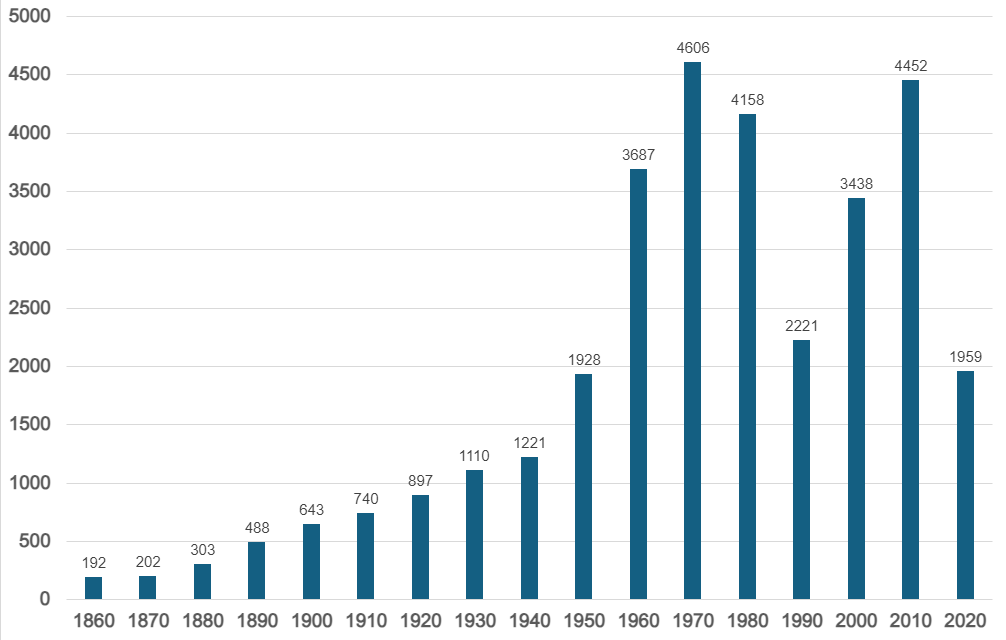
\includegraphics[width=1\textwidth]{./chapter/musical_composition/BarChart_of_The_number_of_music_compositions_for_every_10_years.svg.png}
    \vspace{-7pt}
	\caption{Гистограмма количества музыкальных произведений, 
             создаваемых каждое десятилетие во всём мире со второй половины XIX века до настоящего времени}%
	\label{fig:diagram_10_years}%
\end{marginfigure}
%
Рис.~\ref{fig:diagram_10_years} показывает, что до 1890 года (1850--1890 годы) 
количество написанных музыкальных произведений невелико. 
После 1890 года (1890--1970 годы) начинается резкий подъём числа новых произведений 
и продолжается до нашего времени. 
Такое увеличение музыкальных произведений можно объяснить тем, 
что со временем появляются новые жанры и новые устройства для записи. 
На гистограмме (рис.~\ref{fig:diagram_10_years}) видим два пика: 1960--1990-е и 2000--2010-е.

\todoVlad{
На рис.~\ref{fig:diagram_10_years} нужно сделать крупные подписи по обеим осям (название оси и числа). 
Можете доработать в графическом редакторе. 
Не забудьте новые версии рисунков загружать на Викисклад 
(можно поверх старых, чтобы не писать заново описание файла) 
и новые рисунки включайте в свою страницу в Викиверситете, то есть сюда: 
\textit{Программирование Викиданных/Музыкальные композиции}.

\vspace{12pt}
Сейчас на этом рисунке есть тонкая полоса слева.  
Сделайте crop, пожалуйста, в итоговой картинке. 
}
\answerVlad{...}



\section{Количество музыкальных произведений по десятилетиям в России}

Добавим в запрос~\ref{lst:MusicEvery10Years} страну происхождения 
музыкальных произведений (Российская империя, СССР и Россия), 
а~ограничение по годам в строке 9 уберём. 
Получим запрос~\ref{lst:MusicRussia10Years}, 
подсчитывающий сколько отечественных музыкальных произведений было написано 
в каждом десятилетии с середины XIX века до настоящего времени.


\newpage

\marginnote[4\baselineskip]{%
        \label{question:music_unique}
        \MarginQuestion
       Как избавится от дубликатов в запросе~\ref{lst:MusicRussia10Years}, то есть чтобы независимо от числа композиторов, музыкальные произведения не повторялись. 
        См. ответ~\ref{lst:Number_of_unique_musical_compositions} на с.~\pageref{answer:music_unique_answ}.
}

\begin{lstlisting}[ 
    language=SPARQL,
    caption={\href{https://w.wiki/9q9m}
                  {Подекадное количество отечественных музыкальных произведений\\
                   с~известным автором}\protect\footnotemark},
    label=lst:MusicRussia10Years,
    xleftmargin=18pt,
    numbers=left,
    ]
# List of music written in Russia by composer with date of publication
SELECT DISTINCT ?music ?musicLabel ?year ?year10 ?countryLabel 
       ?composer ?composerLabel WHERE 
{                  # Russian Empire, USSR, Russia
    VALUES ?country {wd:Q34266 wd:Q15180 wd:Q159}
    ?music (*@\hl{wdt:P17|wdt:P495}@*) ?country. # has country or country of origin  
    
           # instance of subclasses of musical work/composition
    ?music wdt:P31 [wdt:P279* wd:Q105543609];
           wdt:P86 ?composer;  # written by composer
           wdt:P577 ?date.     # has publication date
    
    BIND(YEAR(?date) AS ?year)
    BIND((FLOOR(?year / 10)) * 10  AS ?year10)
    
    SERVICE wikibase:label { bd:serviceParam wikibase:language "ru, en" }
}
\end{lstlisting}%
\footnotetext{Получено: 125 русских композиций с~известным автором, 145~--- без автора. 
Ссылка на SPARQL-запрос: \href{https://w.wiki/9q9m}{https://w.wiki/9q9m}.}

В запросе~\ref{lst:MusicRussia10Years} в строке 6 
есть интересная конструкция \lstinline{wdt:P17|wdt:P495}, состоящая из трёх частей:
\begin{enumerate}
\item свойство \wdProperty{17}{<<государство>>}; 
\item свойство \wdProperty{495}{<<страна происхождения>>}; 
\item вертикальная палочка (\emph{пайп}, англ. pipe), выполняющая роль союза <<или>>. 
    Палочка означает, что должно выполняться хотя бы одно из разделяемых ею свойств.
\end{enumerate}
\index{SPARQL!pipe (или)}%      \index{SPARQL!\Vert pipe}

То есть эта конструкция требует от переменной \lstinline|?music|, 
чтобы <<страной происхождения>> музыкальной композиции была Россия или её предшественники, 
или чтобы она имела отношение к~России посредством свойства <<государство>>. 

Теперь с помощью запроса~\ref{lst:MusicRussia10YearsGraph} увидим на рис.~\ref{fig:RussianMusic10years} 
количество музыкальных произведений, 
создаваемых каждое десятилетие в~России и СССР с~XIX века до~настоящего времени. 
В~основном это только те~композиции, о~которых есть статьи в~Википедии на~каком-либо языке. 


\begin{lstlisting}[ 
    language=SPARQL,
    caption={\href{https://w.wiki/9qAY}
                  {График количества отечественных музыкальных произведений\\
                   с~известным автором за каждые 10 лет}\protect\footnotemark},
    label=lst:MusicRussia10YearsGraph,
    texcl,
    ]
# Chart of music written in Russia by composer with date of publication
#defaultView:BarChart
SELECT (STR(?year10) AS ?date_str) (COUNT(?music) AS ?count) WHERE {
                  # Russian Empire, USSR, Russia
    VALUES ?country {wd:Q34266 wd:Q15180 wd:Q159}
    ?music wdt:P17|wdt:P495 ?country. # has country or country of origin  
    
           # instance of subclasses of musical work/composition
    ?music wdt:P31 [wdt:P279* wd:Q105543609];
           wdt:P86 ?composer;  # written by composer
           wdt:P577 ?date.     # has publication date
    
    BIND(YEAR(?date) AS ?year)
    BIND((FLOOR(?year / 10)) * 10  AS ?year10)
}
GROUP BY ?year10 ORDER BY ?year10
\end{lstlisting}%
\footnotetext{Получено: 19 декад с числом музыкальных произведений. 
    Ссылка на SPARQL-запрос: \href{https://w.wiki/9qAY}{https://w.wiki/9qAY}.}

\begin{marginfigure}[0\baselineskip]
	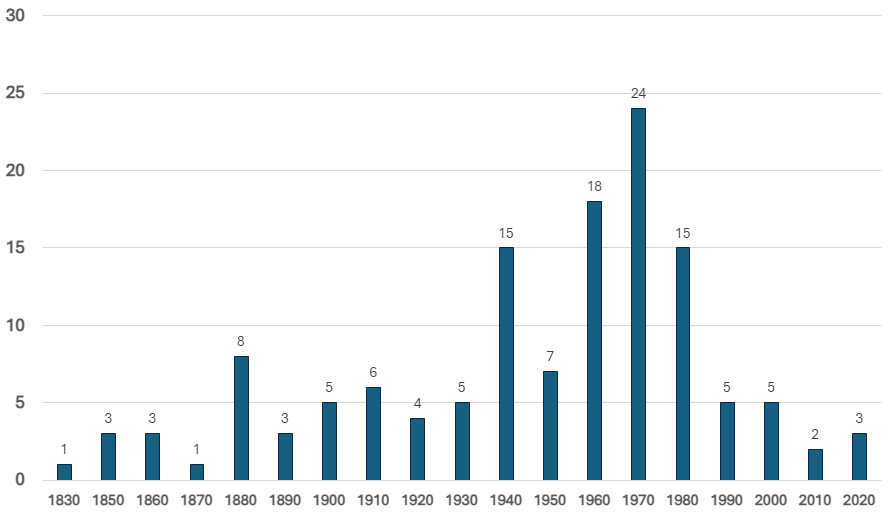
\includegraphics[width=1\textwidth]{./chapter/musical_composition/Graph_music_in_Russia_10.png}
    \vspace{-10pt}
	\caption{Гистограмма количества музыкальных произведений, 
             создаваемых каждое десятилетие в России и СССР с~XIX века до~настоящего времени}%
	\label{fig:RussianMusic10years}%
\end{marginfigure}


Если в~запросе~\ref{lst:MusicRussia10Years} мы получаем список требуемых композиций, 
то   в~запросе~\ref{lst:MusicRussia10YearsGraph} это те же композиции, но уже безымянные, 
разбитые по~десятилетиям, и всё, что нас интересует для построения рис.~\ref{fig:RussianMusic10years},~--- 
это число композиций за десять лет. 
В~этих двух запросах мы искали <<российскую музыку>>, то есть композиции со свойствами 
\wdProperty{17}{<<государство>>} или 
\wdProperty{495}{<<страна происхождения>>}, имеющими значение <<Россия>>. 
Получилось мало, всего 125 музыкальных композиций. 

Проанализировав несколько отечественных песен, таких как: 
\wdqName{<<Песня без слов (Кино)}{101001315}, 
\wdqName{<<Музыка нас связала}{105724079}, 
\wdqName{<<Розовое вино}{57744615}, 
не~попавших в~результаты запроса~\ref{lst:MusicRussia10Years}, стало понятно, 
что у~этих произведений отсутствует свойство \wdProperty{495}{<<Cтрана происхождения>>} и свойство \wdProperty{17}{<<государство>>}. 
То~есть далеко не~у~всех композиций заполнены свойства, 
связанные со~страной. 
Предположим, что для увеличения музыкального охвата нужно перейти от~<<государственности>> музыки 
к~гражданству автора музыки. 
То есть строим последовательность: музыка $\rightarrow$ композитор $\rightarrow$ 
гражданство $\rightarrow$ Российская Империя или СССР, или Россия.
В~соответствии с этой последовательностью построили запрос \href{https://w.wiki/9wcE}
                                                                {https://w.wiki/9wcE}, 
который нашёл в дюжину раз больше музыкальных композиций~--- 1552 по~данным на~2024 году. 
Преобразуем запрос \href{https://w.wiki/9wcE}
                        {https://w.wiki/9wcE} в запрос~\ref{lst:RussianComposers10years} 
для рисования гистограммы подекадного числа музыкальных композиций, 
написанных отечественными авторами (рис.~\ref{fig:RussianComposers10years}). 

Предположение оправдалось, количество композиций отечественных авторов 
(рис.~\ref{fig:RussianComposers10years}) 
по~некоторым декадам в~десятки раз превосходит 
количество отечественных музыкальных произведений (рис.~\ref{fig:RussianMusic10years}).


\begin{marginfigure}[0\baselineskip]
	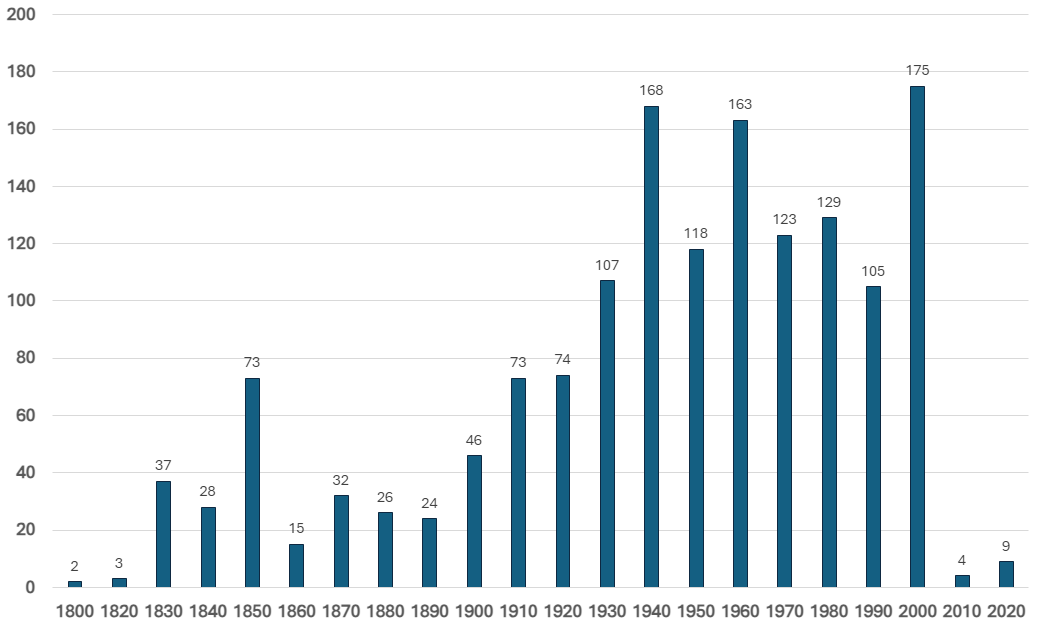
\includegraphics[width=1\textwidth]{./chapter/musical_composition/Graph_music_by_composers_from Russia_10.png}
    \vspace{-7pt}
	\caption{Подекадный график количества музыкальных произведений, написанных отечественными авторами}%
	\label{fig:RussianComposers10years}%
\end{marginfigure}


\begin{lstlisting}[ 
    language=SPARQL,
    caption={\href{https://w.wiki/9qB7}
                  {Количество музыкальных произведений, написанных композиторами из Росии и СССР 
                   за каждые 10 лет}\protect\footnotemark},
    label=lst:RussianComposers10years,
    texcl,
    ]
# Chart of music written by Russian composer with date of publication
#defaultView:BarChart
SELECT (STR(?year10) AS ?date_str) (COUNT(?music) AS ?count) WHERE {
    
           # instance of subclasses of musical work/composition
    ?music wdt:P31 [wdt:P279* wd:Q105543609];
           wdt:P86 ?composer;  # written by composer
           wdt:P577 ?date.     # has publication date
    
                  # Russian Empire, USSR, Russia
    VALUES ?country {wd:Q34266 wd:Q15180 wd:Q159}.
    ?composer wdt:P27 ?country. # citizenship is Russian
  
    BIND(YEAR(?date) AS ?year)
    BIND((FLOOR(?year / 10)) * 10  AS ?year10)
}
GROUP BY ?year10
ORDER BY ?year10
\end{lstlisting}%
\footnotetext{Ссылка на SPARQL-запрос: \href{https://w.wiki/9qB7}{https://w.wiki/9qB7}.}




\newpage

\begin{marginfigure}[0\baselineskip]
	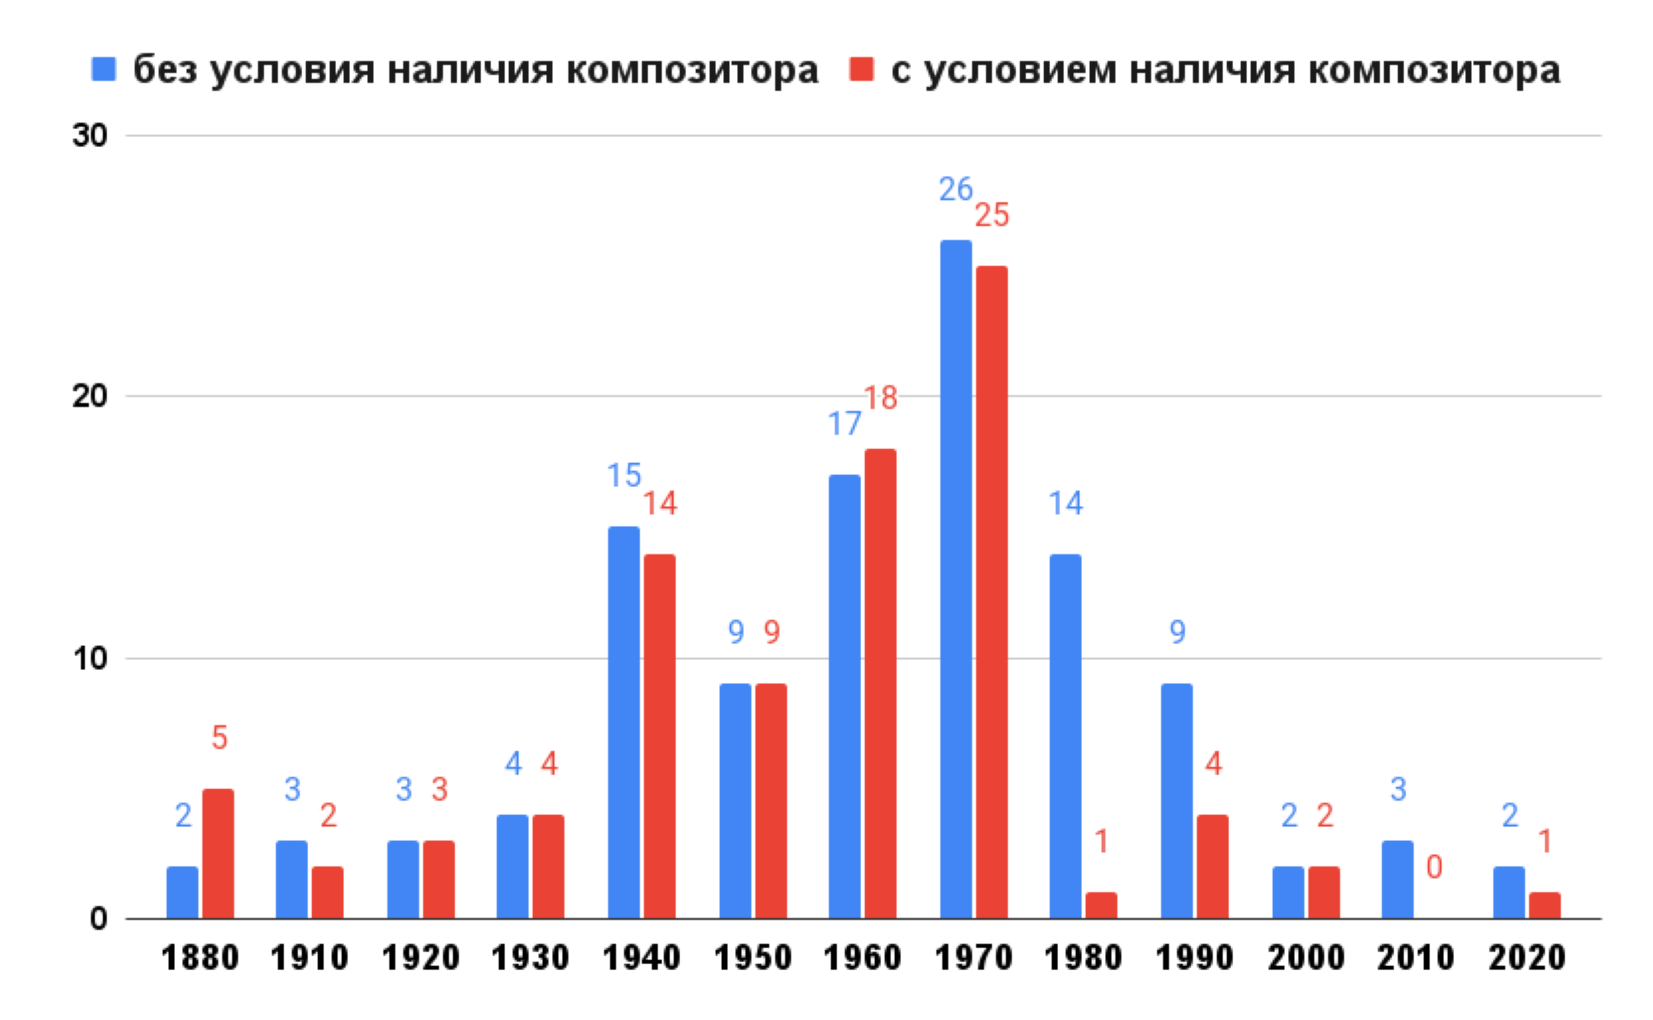
\includegraphics[width=1\textwidth]{./chapter/musical_composition/graph_of_comparison_of_readings.png}
	\caption{Сравнение числа музыкальных композиций по десятилетиям в России,  
             с~указанием композитора и~с~неизвестным автором}%
	\label{fig:CompareRuMusComposerWithout}%
\end{marginfigure}

Строка~10 запроса~\ref{lst:MusicRussia10Years}~---  
\lstinline|wdt:P86 ?composer;|~--- 
требует наличия композитора у музыкального произведения. 
Если убрать эту строку (модифицированный запрос \href{https://w.wiki/9vh2}
                                                     {https://w.wiki/9vh2}), 
то получим произведения как с~композиторами, так и~без~них. 

Сравним результаты обоих скриптов на рис.~\ref{fig:CompareRuMusComposerWithout}. 
Эта диаграмма показывает, что модифицированный запрос 
в основном выдаёт больше или столько же результатов, 
как и~исходный запрос~\ref{lst:MusicRussia10Years}, 
что логично, потому что модифицированный запрос не имеет обязательного условия наличия композитора. 


\todoVlad{
    Мы перешли от запроса~\ref{lst:MusicRussia10Years} к запросу~\ref{lst:RussianComposers10years} 
    (от рис.~\ref{fig:RussianMusic10years} к рис.~\ref{fig:RussianComposers10years}) 
    и десятикратно увеличили число музыкальных композиций за декаду 
    (не 1--24, а больше 100). 


    В начале этой страницы написано: 
    <<Строка~10 запроса~\ref{lst:MusicRussia10Years}~---  \lstinline|wdt:P86 ?composer;|~---...>>. 
    Всё верно, но я предлагаю для рисования рис.~\ref{fig:CompareRuMusComposerWithout} 
    взять запрос~\ref{lst:RussianComposers10years}. 

    То есть рис.~\ref{fig:CompareRuMusComposerWithout} должен существенно вырасти по вертикали 
    и запрос для его создания должен измениться 
    (т. е. не отечественные композиции, а отечественные авторы музыки). 

    Два абзаца выше немного обновятся. 

    Кстати, оставьте рис.~\ref{fig:CompareRuMusComposerWithout}, 
    а новый (с б\'{о}льшими значениями) добавьте ниже. 
    Будет интересно сравнить - изменятся ли пики и волны? 
}
\answerVlad{Ответ: ...}

Но есть исключения, например: 1880-е, 1960-е. 
Посмотрим список музыкальных композиции с~помощью запроса \href{https://w.wiki/9vi8}
                                                               {https://w.wiki/9vi8}. 
За 1880 год этот запрос выдает 8~результатов: 
\wdqName{<<Всенощное бдение>>}{16002554} (1 раз), 
\wdqName{<<Ромео и Джульетта>>}{763716} (1 раз), 
\wdqName{<<Реве та стогне Дніпр широкий>>}{12147183} (1 раз), 
\wdqName{<<Молитва за Украину>>}{7239019} (1 раз), 
\wdqName{String Quartet on the Theme B-la-F}{18660379} (4 раза). 
Вторая композиция повторяется 4 раза, поскольку в этом музыкальном объекте указаны 4~композитора. 






\newpage
\section{Количество музыкальных произведений по жанрам}
\label{chapter:Number-of-musical-works-by-genre}

Найдём, в каких жанрах были написаны музыкальные произведения 
в пиках графика (рис.~\ref{fig:diagram_10_years}) 
и~изобразим жанры на~круговой диаграмме (рис.~\ref{fig:Genre_Chart_1960_—_1990}), 
полученной по запросу~\ref{lst:music_in_genres_1960-1990}. 
Рассмотрим первый пик, приходящийся на~1960--1990-е годы, назовём этот пик <<Первая волна>>.

\begin{marginfigure}[0\baselineskip]
	\includegraphics[width=1\textwidth]{./chapter/musical_composition/Genre_Chart_1960_—_1990.png}
	\caption{Круговая диаграмма музыкальных жанров за 1960--1990 годы во всем мире}%
	\label{fig:Genre_Chart_1960_—_1990}%
\end{marginfigure}

\begin{lstlisting}[ 
    language=SPARQL,
    caption={\href{https://w.wiki/9aGd}
                  {Количество музыкальных произведений в каждом жанре в промежутке с 1960 по 1990 годы.}\protect\footnotemark},
    label=lst:music_in_genres_1960-1990,
    xleftmargin=18pt,
    numbers=left,
    ]
# Count of pieces of music in each subclass
SELECT ?type (COUNT(?music) AS ?count) ?typeLabel WHERE {
  {?type wdt:P31 wd:Q107487333} UNION 
  {?type wdt:P31 wd:Q188451} . # subclass of composed musical work
  ?music wdt:P31 ?type;     # is instance of this subclass
         wdt:P577 ?date;    # has publication date
         wdt:P86 ?composer. # written by composer
  BIND(YEAR(?date) AS ?year)
  FILTER(?year > 1960)        
  FILTER(?year < 1990)
  SERVICE wikibase:label { bd:serviceParam wikibase:language "ru, en" }
}
GROUP BY ?type ?typeLabel
ORDER BY DESC (?count)
\end{lstlisting}%
\footnotetext{Получено: \num{15} подклассов на 2024 год. Ссылка на SPARQL-запрос: \href{https://w.wiki/9aGd}{https://w.wiki/9aGd}.}

Строки 7 и 8 в запросе~\ref{lst:music_in_genres_1960-1990} определяют промежуток времени с 1960 года до 1990 год, который является <<первой волной>>, в этом промежутке будет производиться поиск музыкальных произведений по дате их публикации.

\todoVlad{
Зачем в запросе~\ref{lst:music_in_genres_1960-1990} есть строка
\lstinline|wdt:P86 ?composer|? 
Если её убрать, то результатов будет больше. 

\vspace{12pt}
Меня смущало, что на этом <<кружке>> есть духовные песни, а всякого панка, рока и джаза нет. 
Странно. Я взял любую известную рок-музыку, посмотрел её свойства, и у меня получился такой 
весёлый скрипт: \href{https://w.wiki/9wuk}
                     {https://w.wiki/9wuk}. Этот запрос работает долго, но со второй попытки выдал результат.\\
Если сможете, то ускорьте его работу.\\
Если сможете, то объедините его с запросом~\ref{lst:music_in_genres_1960-1990}. 

То же замечание к следующему запросу и к следующей круговой диаграмме 
(там где второй пик графика).\\ 
Кстати, если следующий запрос меняется только в двух строчках, то сократите листинг, 
оставьте только эти две строчки, а выше и ниже сделайте по одной строчке с многоточием.
} 
\answerVlad{Ответ: ...}



\newpage
Теперь рассмотрим второй пик графика~\ref{fig:diagram_10_years}: 2000-е и 2030-е (<<вторая волна>>) рис.~\ref{fig:Genre_Chart_2000_—_2030}, пользуясь запросом~\ref{lst:music_in_genres_after2020}.

\begin{lstlisting}[ language=SPARQL,
                    caption={\href{https://w.wiki/9aJC}{ Количество музыкальных произведений в каждом жанре в промежутке с 2000 по 2030 годы.}\protect\footnotemark},
                    label=lst:music_in_genres_after2020,
                    texcl 
                    ]
# Count of pieces of music in each subclass
SELECT ?type (COUNT(?music) AS ?count) ?typeLabel WHERE {
  {?type wdt:P31 wd:Q107487333} UNION 
  {?type wdt:P31 wd:Q188451} . # subclass of composed musical work
  ?music wdt:P31 ?type;    # is instance of this subclass
         wdt:P577 ?date;    # has publication date
         wdt:P86 ?composer.  # written by composer
    BIND(YEAR(?date) AS ?year)
  FILTER(?year > 2000)        
  FILTER(?year < 2030)
  SERVICE wikibase:label { bd:serviceParam wikibase:language "ru, en". }
}
GROUP BY ?type ?typeLabel
ORDER BY DESC (?count)
\end{lstlisting}%
\footnotetext{Получено: \num{21} подкласс на 2024 год. Ссылка на SPARQL-запрос: \href{https://w.wiki/9aJC}{https://w.wiki/9aJC}.}

\begin{marginfigure}[0\baselineskip]
	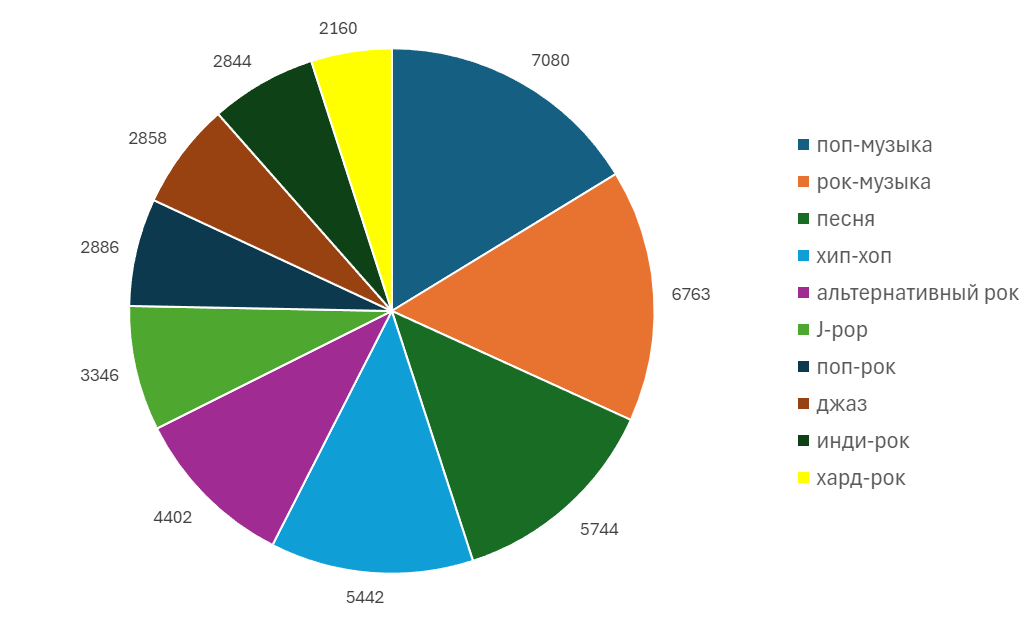
\includegraphics[width=1\textwidth]{./chapter/musical_composition/Genre_Chart_2000-2030.png}
	\caption{Круговая диаграмма числа музыкальных жанров за 2000--2030 годы во всем мире}%
	\label{fig:Genre_Chart_2000_—_2030}%
\end{marginfigure}

Из результатов запроса~\ref{lst:music_in_genres_1960-1990} 
и~запроса~\ref{lst:music_in_genres_after2020}, можем сделать вывод, 
что жанры музыкальных произведений первого пика, не отличаются от жанров второго. 
На второй диаграмме~\ref{fig:Genre_Chart_2000_—_2030}, видим, что 95,5\,\% музыкальных произведений написаны в жанре <<песня>>. В жанре <<духовная песня>> количество музыкальных произведений по сравнению с рис.~\ref{fig:Genre_Chart_1960_—_1990} уменьшилось почти в 4 раза. А такие музыкальные жанры, как: <<гимн>> и <<музыкальная тема>> на диаграмме~\ref{fig:Genre_Chart_2000_—_2030} по сравнению с диаграммой~\ref{fig:Genre_Chart_1960_—_1990} пропали.




\newpage
\section{Поиск музыкальных лакун в общественном достоянии}

Задача состоит в том, чтобы найти такие музыкальные произведения, 
авторы которых умерли более 70 лет назад, 
и аудиозапись которых отсутствует на Викискладе. 
Найдём и упорядочим такие произведения от самых старых к новым 
с помощью запроса~\ref{lst:music_gaps_in_public_domain}. 
Существует практическая выгода и польза от~такого запроса~\ref{lst:music_gaps_in_public_domain}, 
поскольку видно, какие произведения можно и нужно оцифровывать 
(с~пластинок, кассет) и загружать на~Викисклад для илюстрации статей Википедии.

\begin{lstlisting}[ 
    language=SPARQL,
    caption={\href{https://w.wiki/9qGu}
                  {Отсутствующие аудиозаписи музыкальных произведений,\\
                  авторы которых умерли более 70 лет назад }\protect\footnotemark},
    label=lst:music_gaps_in_public_domain,
    texcl,
    numbers=none
    ]
# Search music gaps in public domain
SELECT ?music ?musicLabel (YEAR(?date) as ?year) WHERE 
{
  ?music wdt:P31 wd:Q105543609; # is musical work/composition
         wdt:P86 ?composer;     # has a composer
         wdt:P577 ?date.        # has a publication date
  MINUS {?music wdt:P51 []}.	# skip music without audio 
  
  ?composer wdt:P570 ?death.    # composer has a date of death
  FILTER(?death<"1953-01-01T00:00:00Z"^^xsd:dateTime) # composer passed away > 70 years
  FILTER(?date < "1953-01-01T00:00:00Z"^^xsd:dateTime) # music published > 70 years ago
  SERVICE wikibase:label { bd:serviceParam wikibase:language "ru,en" }
}
ORDER BY ASC(?date)
\end{lstlisting}%
\footnotetext{Получено: \num{3771} запись на 2017 год, \num{4273} записи на 2023 год и \num{4467} записей на 2024 год. Ссылка на SPARQL-запрос: \href{https://w.wiki/9qGu}{https://w.wiki/9qGu}.}

В России общественное достояние включает природные ресурсы, культурные объекты, 
научные достижения и образовательные ресурсы, 
предназначенные для общего пользования и подлежащие сохранению в соответствии с законодательством. 
В общем случае произведение переходит в общественное достояние в России, 
если с года смерти его автора прошло 70 лет. 
Кроме того, существует <<правило 70+4>>, согласно которому лица, 
трудившиеся или участвовавшие в Великой Отечественной войне, 
могут рассчитывать на приоритет в использовании общественных ресурсов\sidenote{%
%
    URL: \href{https://ru.wikipedia.org/?curid=31363}
              {https://ru.wikipedia.org/wiki/Общественное\_достояние}.%
%
}.            



\section{Полнота Викиданных}

Проанализируем полноту Викиданных. 
Сравним количесво уникальных композиторов, предоставленных в Викиданных, 
с числом композиторов по другим источникам. 
Также проверим, как изменяется полнота Викиданных со временем, 
сравнив результаты запроса~\ref{lst:BubbleComposers} за~2017 год, 
рис.~\ref{fig:Composers2017} и за~2023 год, рис.~\ref{fig:Composers2023}.

На сайте  
\href{https://ru.wikipedia.org/?curid=1362802}
     {<<Музыкального словаря Гроува>>} 
представлена информация о~\num{33000} композиторов и музыкантов\sidenote{%
                    URL: \href{https://www.oxfordmusiconline.com/page/about-gmo/about-grove-music-online}
                              {https://www.oxfordmusiconline.com/page/about-gmo/about-grove-music-online}.}. 
По данным категории 
\href{https://ru.wikipedia.org/?curid=155531}
     {<<Композиторы по алфавиту>>} 
Русской Википедии существует \num{7800} композиторов\sidenote{%
                    URL: \href{https://ru.wikipedia.org/?curid=155531}
                              {https://ru.wikipedia.org/?curid=155531}.}. 
По данным категории 
\href{https://en.wikipedia.org/?curid=6921880}
     {List of composers by name} 
Английской Википедии существует \num{4958} композиторов\sidenote{%
                    URL: \href{https://en.wikipedia.org/?curid=6921880}
                              {https://en.wikipedia.org/?curid=6921880}.}.

Количество музыкальных композиций с заполненным свойством \wdProperty{86}{композитор} равно \num{3862}, 
что показывает нам запрос \href{https://w.wiki/56Rc}{https://w.wiki/56Rc}, 
и~это с~учётом того, что один композитор мог написать несколько музыкальных произведений. 
Например, \href{https://ru.wikipedia.org/wiki/Моцарт,_Вольфганг_Амадей}{Вольфганг Амадей Моцарт} 
написал 95 произведений, что существенно снижает количество уникальных композиторов. 
Полученное число 3862, 
из результатов запроса \href{https://w.wiki/56Rc}{https://w.wiki/56Rc}, меньше, 
чем количество композиторов из Русской и Английской Википедии и существенно меньше, 
чем количество композиторов из \href{https://ru.wikipedia.org/wiki/Музыкальный_словарь_Гроува}{<<Музыкального словаря Гроува>>}, что говорит нам о неполноте Викиданных.


\todoVlad{Скрипты и числа выше устарели. Возможно, скрипты потребуют переделки.}
\answerVlad{Не получается исправить скрипты. Поменял \wdqName{<<музыкальная композиция>>}{207628} 
на \wdqName{<<музыкальное произведение/композиция>>}{105543609}>>. 
Но при выполнении запроса пишет, что запрос занял слишком много времени.}
\todoVlad{
    Ладно, в будущем сам переделаю. Это уже пустяки по сравнению с остальной работой.}


\begin{marginfigure}[-0\baselineskip]
  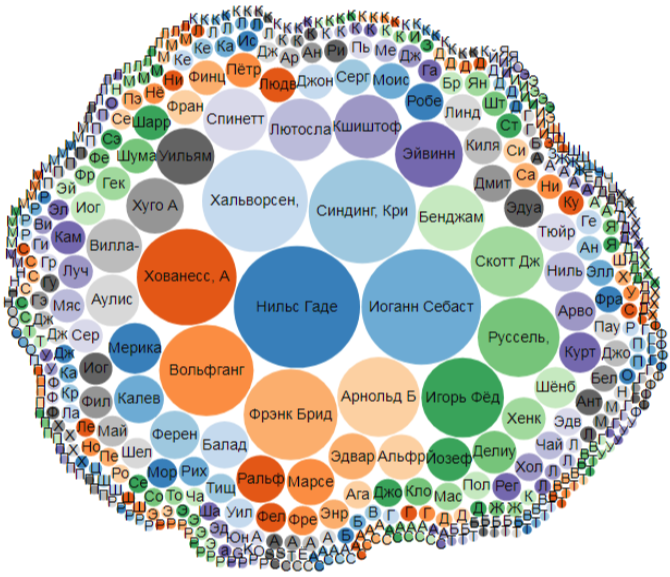
\includegraphics[width=\textwidth]{./chapter/musical_composition/Composer_all_2017.png}
  \vspace{-7pt}
  \caption[Пузырьковая диаграмма композиторов по количеству написанных композиций на~2017 год]{Пузырьковая диаграмма композиторов по количеству написанных композиций на~2017 год}%
  \label{fig:Composers2017}%
\end{marginfigure}

Запрос \href{https://w.wiki/9arZ}{https://w.wiki/9arZ} 
по~композициям с~заполненным свойством \wdProperty{86}{композитор} 
и~свойством \wdProperty{495}{<<страна происхождения>>}, 
имеющим значения \wdqName{<<Российская империя>>}{34266}, \wdqName{СССР}{15180} или \wdqName{Россия}{159}, 
выдал 176 произведений.


\newpage
Запрос~\ref{lst:BubbleComposers} строит пузырьковую диаграмму композиторов по числу написанных ими произведений.
Мы запускали этот скрипт в 2017 году (рис.~\ref{fig:Composers2017}) 
и~в~2023 году (рис.~\ref{fig:Composers2023}).


\begin{lstlisting}[ 
    language=SPARQL, 
    numbers=none,
    caption={\href{https://w.wiki/9are}
                  {Пузырьковая диаграмма композиторов по~числу музыкальных произведений}\protect\footnotemark},
    label=lst:BubbleComposers,
    texcl,
    numbers=none
    ]
# composers with musical compositions
#defaultView:BubbleChart
SELECT ?composer ?composerLabel (COUNT(*) AS ?count) WHERE {
  ?music wdt:P31 wd:Q105543609; # this composition
               wdt:P86 ?composer.     # was written by the composer
  SERVICE wikibase:label { bd:serviceParam wikibase:language "ru, en" }
}
GROUP BY ?composer ?composerLabel
ORDER BY DESC(?count) ?composerLabel
\end{lstlisting}%
\footnotetext{Получено: \num{773} записи. Ссылка на SPARQL-запрос: \href{https://w.wiki/9are}{https://w.wiki/9are}.}

Размер круга означает количество написанных музыкальных композиций. Диаграмма показывает, что у одних композиторов значительно больше композиций чем у других. В~первую пятерку входят \href{https://ru.wikipedia.org/wiki/Гаде,_Нильс}{Нильс Гаде} (\num{173} композиции), \href{https://ru.wikipedia.org/wiki/Бах,_Иоганн_Себастьян}{Иоганн Себастьян Бах} (\num{155} композиций), \href{https://ru.wikipedia.org/wiki/Синдинг,_Кристиан_Август}{Кристиан Август Синдинг} (\num{125} композиций), \href{https://ru.wikipedia.org/wiki/Хальворсен,_Юхан}{Юхан Хальворсен} (\num{121} композиция), \href{https://ru.wikipedia.org/wiki/Хованесс,_Алан}{Алан Хованесс} (\num{108} композиций).

%
%
\begin{marginfigure}[-6\baselineskip]
  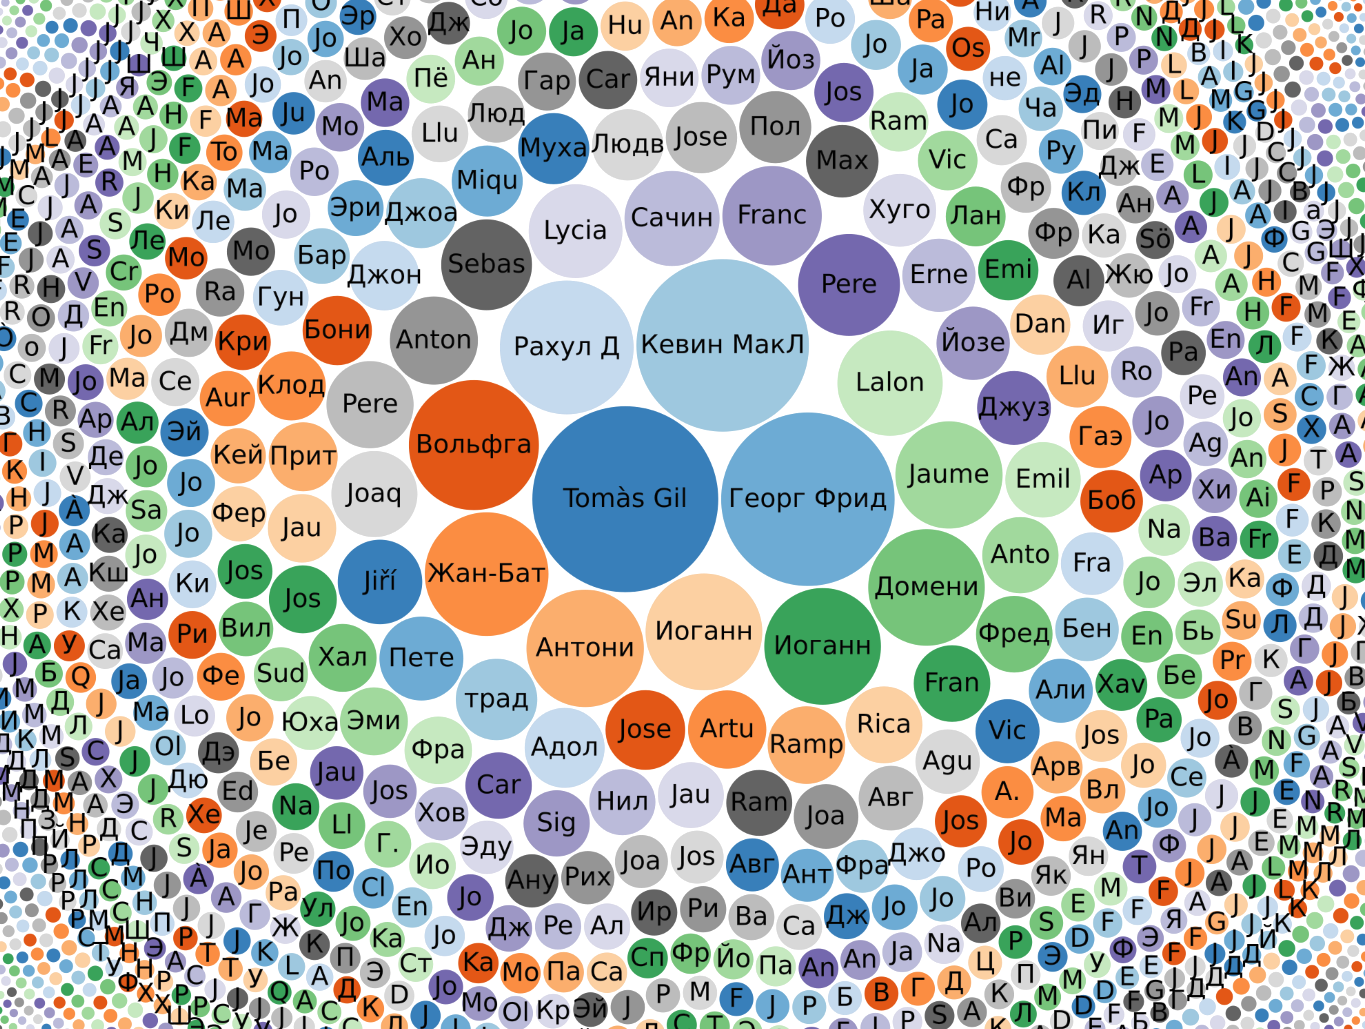
\includegraphics[width=\textwidth]{./chapter/musical_composition/Composer_all_2023_box.png}
  \vspace{-7pt}
  \caption[Пузырьковая диаграмма композиторов по количеству написанных композиций на~2023 год]
    {Фрагмент диаграммы композиторов по количеству написанных произведений на~2023 год}%
  \label{fig:Composers2023}%
\end{marginfigure}

Диаграмма~\ref{fig:Composers2023} за 2023 год позывает, 
как изменилось количество написанных композиций у различный композиторов. 
Чтобы рассмотреть подробнее, 
добавим в конец запроса~\ref{lst:BubbleComposers} строку  \lstinline|LIMIT 12|, 
чтобы ограничить количество записей до 12, 
получим следующий запрос \href{https://w.wiki/8A2h}{https://w.wiki/8A2h}, 
результат на рис.~\ref{fig:12composers}. 

Сравним результаты за~2017 год и за~2023 год.
По сравнению с 2017 годом в первую пятёрку входят 
\href{https://ca.wikipedia.org/wiki/Tomàs_Gil_i_Membrado}{Томас Хиль Мембрадо} 
(\num{1437} композиций), 
\href{https://ru.wikipedia.org/wiki/Гендель,_Георг_Фридрих}{Гендель Георг Фридрих} (\num{1251} композиция), 
\href{https://ru.wikipedia.org/wiki/Маклауд,_Кевин}{Маклауд Кевин} (\num{1237} композиций), 
\href{https://en.wikipedia.org/wiki/R._D._Burman}{Рахул Дев Бурман} (\num{744} композиции), 
\href{https://ru.wikipedia.org/wiki/Моцарт,_Вольфганг_Амадей}{Вольфганг Амадей Моцарт} (\num{703} композиции). 
Исходя из данных диаграмм~\ref{fig:Composers2017} и ~\ref{fig:Composers2023}, 
можно сделать вывод, что появились новые композиторы, 
которые имеют значительно больше композиций. 
При этом у такого классика, как 
\href{https://ru.wikipedia.org/?curid=17950}{Иоганн Себастьян Бах}, 
число композиций увеличилось за эти годы на 411 и составило 566. 


\newpage
\begin{marginfigure}
  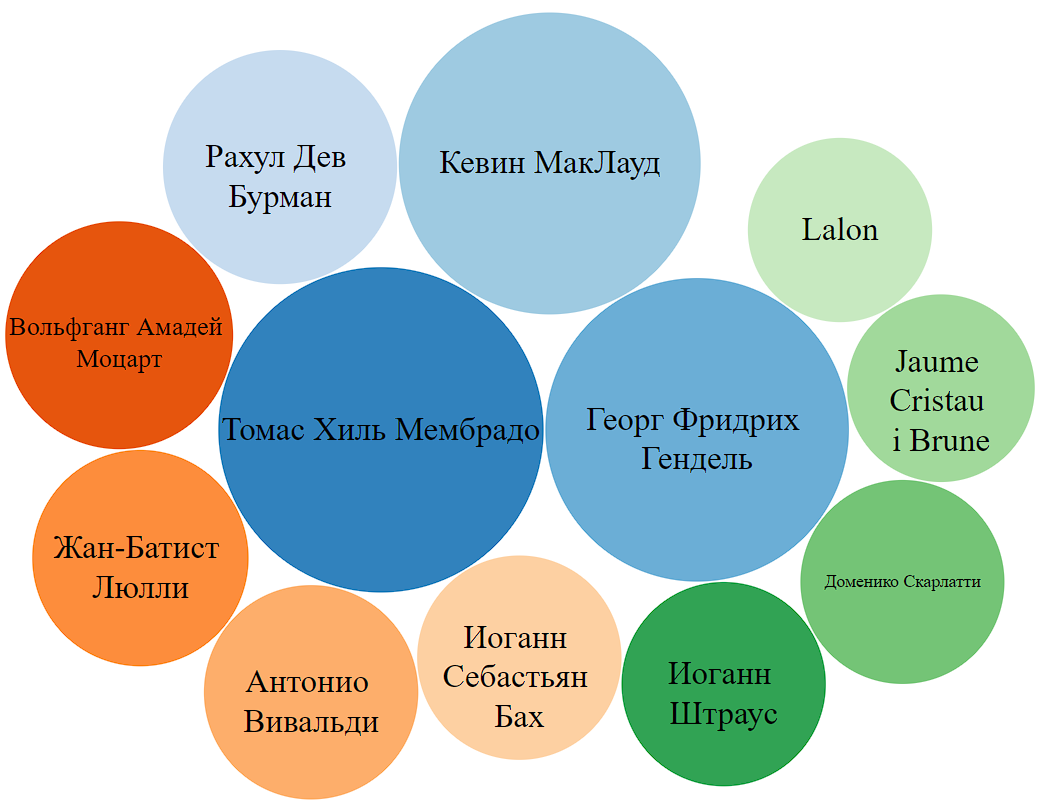
\includegraphics[width=\textwidth]{./chapter/musical_composition/Composers_12_at_2023.png}
  \caption[Диаграмма 12 композиторов с наибольшим количеством написанных музыкальных композиций на~2023 год]
          {Пузырьковая диаграмма 12 композиторов с наибольшим количеством написанных музыкальных композиций на~2023 год}%
  \label{fig:12composers}%
\end{marginfigure}


\section{Упражнения}
\begin{enumerate}
    \item Найти список музыкальных композиций, созданных во время эпохи классицизма (XVII--XVIII века).
Используйте свойство \wdProperty{571}{<<дата создания>>}.
    \item Найти композитора, который написал больше симфоний, чем остальные. 
    Используйте свойства \wdProperty{31}{экземпляр}, \wdProperty{86}{композитор}
        и объект \wdqName{симфония}{9734}.
    item Построить гистограмму, на которой отображается количество музыкальных композиций 
        группы The Beatles по году публикации.
        Используйте свойства: <<\wdProperty{175}{исполнитель}>>, <<\wdProperty{577}{дата публикации}>>. 
%        
        \label{question:TheBeatles_quest}
        (См. ответ %~\ref{lst:TheBeatles} 
         на с.~\pageref{answer:TheBeatles_answ}).

     \item Найти список музыкальных жанров, которые входили в семёрку первых 
         (по количеству музыкальных композиций) хотя бы для одного 
         десятилетия на протяжении всей истории. 
         Подсчитать число музыкальных композиций по этим жанрам для всех десятилетий, 
         представить это на графике. 
         Этот график будет показывать расцвет и падение различных музыкальных жанров. 
\end{enumerate}
